\documentclass[rnd]{mas_proposal}
% \documentclass[thesis]{mas_proposal}

\usepackage[utf8]{inputenc}
\usepackage{amsmath}
\usepackage{amsfonts}
\usepackage{amssymb}
\usepackage{graphicx}

\title{Robot motion planning in dynamic environment: A comparative study}
\author{Dharmin Bakaraniya}
\supervisors{Prof.\ Dr.\ Ervin Prassler\\Dr.\ Cesar Lopez Martinez}

% \thirdpartylogo{path/to/your/image}

\begin{document}

\maketitle

\pagestyle{plain}

\chapter{Introduction}
\begin{itemize}
    \item Mobile robot needs a plan to reach to its desired goal. This plan is provided by motion planning algorithms.
    \item Robot motion planning (RMP) for static environment is not sufficient for most of the application.
    \item Take for example, a robotic wheel chair or robot carrying hospital bed. These robot needs to tackle moving obstacle like patients, other wheel chairs, hospital beds, etc. while safely moving towards its goal.
    \item This type of problem applications need RMP for dynamic environment. 
    \item By solving this problem, we can ensure 
        \begin{itemize}
            \item Safe environment for humans and for robots
            \item Cost effective trasportation of goods
        \end{itemize}
\end{itemize}

\section{Problem Statement}
\begin{itemize}
    \item RMP in dynamic environment needs to perform the following task
        \begin{itemize}
            \item Reach the desired target
            \item Avoid static and moving obstacle
        \end{itemize}
    \item It needs to perform these tasks in \textit{fast} and \textit{efficient} manner.
    \item This work will provide a comparative study on existing approaches for RMP in dynamic environment.
    \item This comparative study will include 
        \begin{itemize}
            \item An in depth literature review of existing approaches
            \item Identifying top solutions
            \item Evaluating these candidates on various benchmark practical test on a real and simulated environment
            \item Identifying the best solution based on the performance measure
        \end{itemize} 
\end{itemize}

\chapter{Related Work}
\begin{itemize}
    \item All the existing approaches have tested their efficiency on different robots and in different test environment.
    \item As the measuring criterion for each of them is different, it becomes an impossible task to determine a clear winner.
    \item There are several existing survey article:
        \begin{itemize}
            \item Mohanan et al. \cite{mohanan2018a} covers 101 research papers that were published between 1985 and 2016 in the field of RMP in dynamic environment. 
                They have addressed all the approaches but a comparative analysis of all the aproaches with their contributions and deficiencies is left to be desired.
            \item Hoy et al. \cite{hoy2015algorithms} provides a survey for algorithms which provide collision free navigation for robots. 
                This survey is not only detailed but also quite broad as it covers obstacle avoidance algorithm as well. 
                Eventhough it provides a comparision between main approaches based on numerous criterion, it still does not evaluate these approaches on a standard uniform test.
            \item Keshmiri et al.\cite{keshmiri2009overview} provides a survey specifically for RMP in dynamic environment. 
                It covers all the approaches presented in research papers published between 1986 and 2008 totalling upto 150 papers. 
                They have provided a comparision on how much contribution has been made in RMP field based on different approach but regarding the actual approaches itself, only a summary of at most 2-3 sentences for each approach is provided.
            \item \cite{fujimura1991motion} and \cite{tsubouchi1996motion} are quite dated and does not cover any state of the art approaches in RMP for dynamic environment.
        \end{itemize}
    \item Existing approaches generally provide critique and deficiencies on their previous works. These are generally helpful but they mostly compare their approach with the existing solutions and only point out the deficincies that they have addressed. Therefore, though these comparisions are helpful, they might not be completely reliable.
\end{itemize}

\section{State of the art}
\subsection{Velocity based}
\begin{itemize}
    \item \textit{Dynamic window approach}: Fox et al. \cite{fox1997dynamic} proposed the original idea for simply optimizing a function which balances robot's distance from goal, distance from nearest obstacle and current velocity. This approach, despite being robust, simple and fast did not work for dynamic environment. 
        Later, Brock et al. \cite{brock1999high} extended this approach for global path planning and for dynamic environments by combining it with NF1 algorithm. 
        This eradicated the problem of local minima. 
        It has been since extended in \cite{seder2007dynamic} and \cite{ogren2005convergent}
    \item \textit{Velocity obstacle (VO)}: Originally developed by Fiorini et al.\cite{fiorini1998motion}, this approach proposes to avoid obstacles by choosing velocity outside \textit{collision cone}.
        This approach unfies the representation for avoiding static and dynamic obstacles.
        This idea has since been transformed to incorporate many scenarios\cite{shiller2010nonlinear}\cite{owen2006a}\cite{owen2005motion}\cite{guy2009clearpath}. 
        For multi robot systems, Van den berg et al.\cite{van2008reciprocal}\cite{van2011reciprocal}\cite{van2006anytime} have extended VO approach.
    \item \textit{ICS based approach}: Inevitable collision states (ICS) \cite{fraichard2004inevitable}\cite{petti2005safe}\cite{martinez2009collision} have proposed a solution to avoid states that has no outcome other than collision. They propose that this states if avoided will ensure that the robot will never collide. They have approached this problem in a mathematical way. They provide a very fast and almost infite look ahead option\cite{mohanan2018a}.

\end{itemize}

\subsection{Roadmap based}
\begin{itemize}
    \item \textit{Probabilistic roadmap}: Hsu et al.\cite{hsu2002randomized} provides an extension of probabilistic roadmap approach by considering kinodynamics of the robot before choosing a motion control.
    \item \cite{van2005roadmap}
\end{itemize}

\subsection{Other}
\begin{itemize}
    \item \textit{Nearness diagram}: \cite{minguez2004nearness}
\end{itemize}


\chapter{Project Plan}

\section{Work Packages}
The bare minimum will include the following packages:
\begin{enumerate}
    \item[WP1] Literature Search
    \item[WP2] Experiments
    \item[WP3] Project Report
\end{enumerate}
Keep in mind that depending on your project, you will probably need to add work packages that are more suited to your projects.

\section{Milestones}
\begin{enumerate}
    \item[M1] Literature search
    \item[M2] Experimental setup
    \item[M3] Experimental Analysis
    \item[M4] Report submission
\end{enumerate}

\section{Project Schedule}
Include a gantt chart here. It doesn't have to be detailed, but it should include the milestones you mentioned above.
Make sure to include the writing of your report throughout the whole project, not just at the end.

\begin{figure}[h!]
    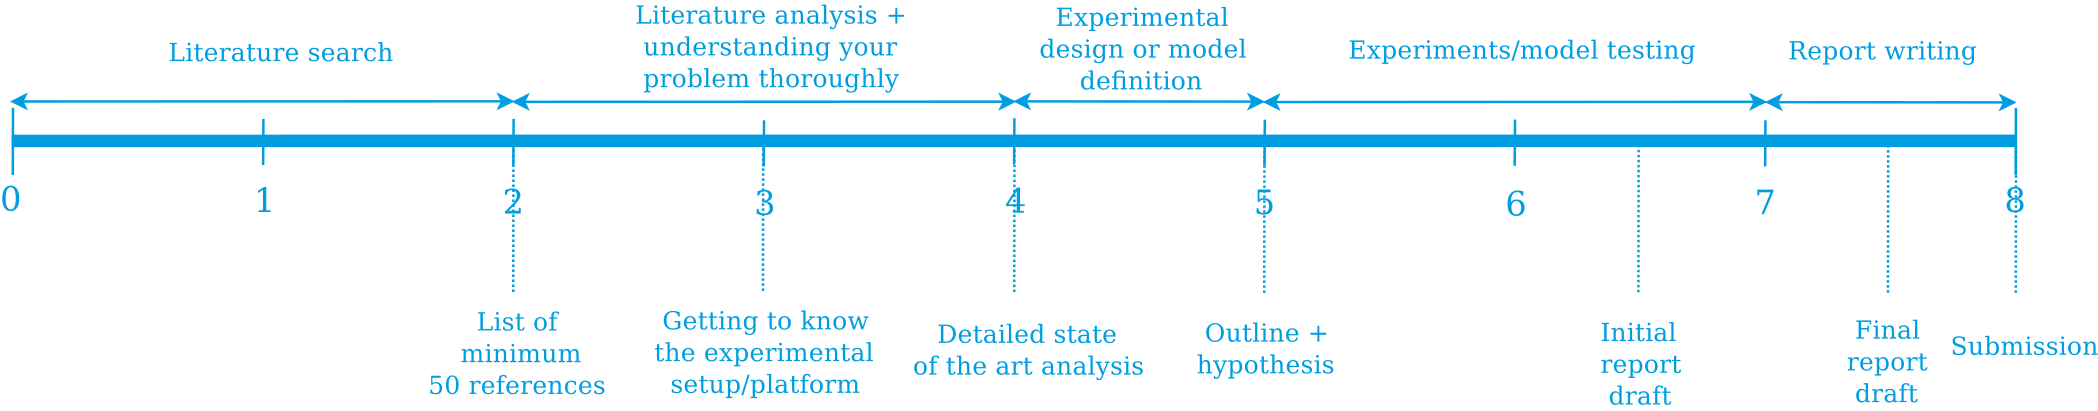
\includegraphics[width=\textwidth]{rnd_deliverable_timeline}
    \caption{}
    \label{}
\end{figure}

\section{Deliverables}
\subsection{Minimum Viable}

\begin{itemize}
    \item Survey
    \item Analysis of state of the art
    \item Simple simulated use case
    \item Demo on youBot or Jenny
\end{itemize}

\subsection{Expected}
\begin{itemize}
    \item Comparation of approaches in the robot
\end{itemize}

\subsection{Desired}
\begin{itemize}
    \item Integration to scenario
\end{itemize}


\nocite{*}

\bibliographystyle{plainnat} % Use the plainnat bibliography style
\bibliography{../myRef.bib} % Use the bibliography.bib file as the source of references




\end{document}
